\newpage
\section{Aufbau und Durchführung}\label{sec:aufbau-und-durchfuehrung}

Der Millikan-Versuch besteht aus einem Plattenkondensator innerhalb einer Kammer. Der detaillierte Versuchsaufbau findet sich in Abbildung~\ref{fig:aufbau}.
\begin{figure}[H]
  \centering
  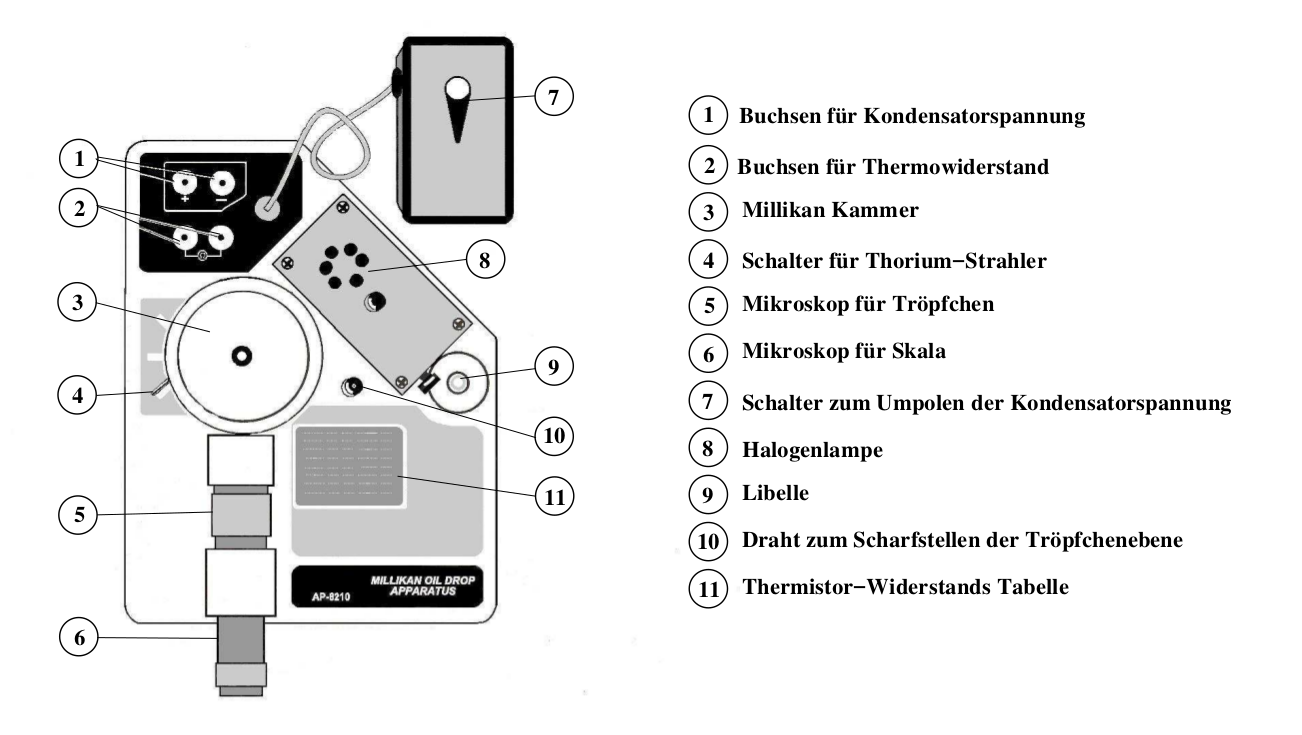
\includegraphics[width=0.4\textheight]{../figures/aufbau.png}
  \caption{Versuchsapparatur zum Millikan-Versuch. [Skript V503]}
\label{fig:aufbau}
\end{figure}

Mit Hilfe eines Zerstäubers können Öltröpfchen durch eine Öffnung in der oberen Platte des Kondensators eingesprüht werden. Ihre Dichte beträgt
\begin{align}
  \rho_{\mathrm{oel}} = 886 \si{\kilogram\per\cubic\m} \; .
\end{align}
Mit einem Mikroskop (siehe Kapitel~\ref{sub:details}) können die Tröpfchen, die durch eine Halogenlampe angestrahlt werden, auf einem Monitor beobachtet werden. Im Hintergrund ist ein Gitter mit einer Kästchenbreite von
\begin{align}
  b = \SI{0.5}{\milli\m}
\end{align}
zu sehen, mit dessen Hilfe die Strecke gemessen werden kann, die sich die Tröpfchen in einer bestimmten Zeit fortbewegen. Die Öltröpfchen sind elektrisch geladen bzw. können mit einem radioaktiven Präparat geladen werden, und können daher durch den Plattenkondensator beeinflusst werden. Die Temperatur innerhalb der Kammer kann über einen Thermowiderstand gemessen werden und wird während der Messung regelmäßig notiert.

Für die Messung wird ein Tropfen ausgewählt, der durch die angelegte Spannung am Kondensator beeinflusst wird. Es wird die Zeit gemessen, die der Tropfen braucht um eine bestimmte Strecke zurückzulegen, dann wird das elektrische Feld umgeschaltet und die Zeit gemessen, die der Tropfen in die entgegengesetzte Richtung benötigt. Die Messung wird so oft wie möglich wiederholt. Dann wird die Geschwindigkeit $v_0$ bestimmt, die der Tropfen bei abgeschaltetem Feld benötigt. Die Messung wird für verschiedene Tröpfchen wiederholt, sowie für verschiedene Spannungen.



%\begin{figure}
%  \centering
%  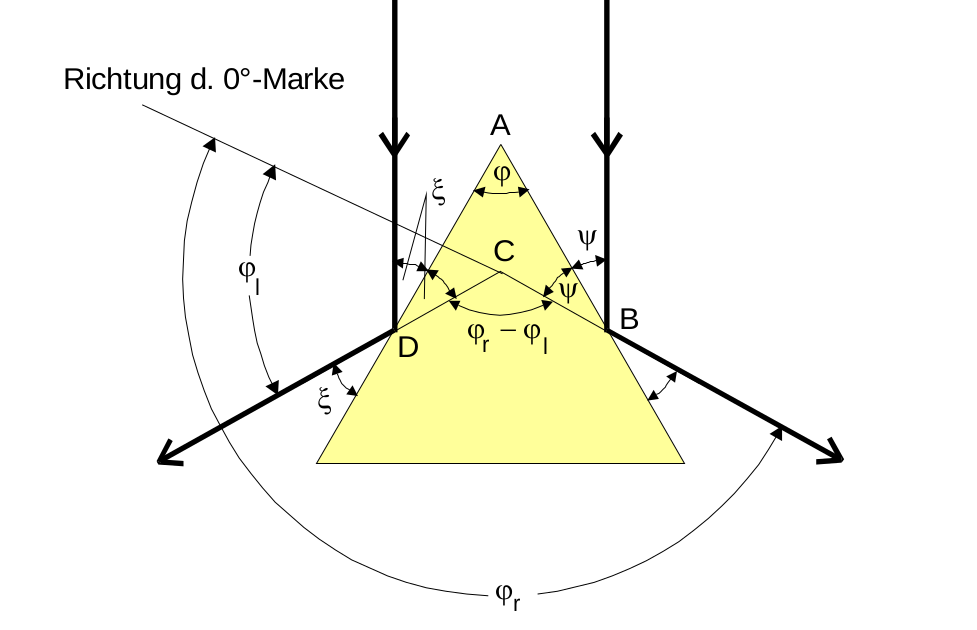
\includegraphics[width=0.4\textheight]{../figures/phi.png}
%  \caption{Schematische Darstellung zur Messung des Winkels~$\varphi$ an der brechenden Kante eines Prismas. [Skript V402]}
%\label{fig:prism}
%\end{figure}
